% Created 2016-08-17 Wed 14:38
\documentclass[tikz]{standalone}

\usepackage[utf8]{inputenc}
\usepackage[T1]{fontenc}
\usepackage{helvet}
\usepackage{../../templates/msc}

\renewcommand{\familydefault}{\sfdefault}

\tikzset{
every picture/.style={
line width=1pt
}}

\usepackage{tikz}
\author{Holger Karl}
\date{\today}
\title{}

\usepackage{ifthen}
\tikzset{
         clear_database/.style={
               cylinder,
               shape border rotate=90,
               aspect=0.25,
               draw
         },
         pics/site/.style n  args={4}{code={

             \ifthenelse{#2=1}{
               \node [draw, rounded corners, fill=blue!20, minimum width=5ex, minimum height=2ex] (d1) {}; }{
               \node [rounded corners, minimum width=5ex, minimum height=2ex] (d1) {}; 
             }
             \ifthenelse{#3=1}{
               \node [above=0cm of d1, draw, rounded corners, fill=green!20, minimum width=5ex, minimum height=2ex] (d2) {}; }{
               \node [above=0cm of d1, rounded corners, minimum width=5ex, minimum height=2ex] (d2) {}; 
             }
             \ifthenelse{#4=1}{
               \node [above=0cm of d2, draw, rounded corners, fill=red!20, minimum width=5ex, minimum height=2ex] (d3) {}; }{
               \node [above=0cm of d2, rounded corners, minimum width=5ex, minimum height=2ex] (d3) {}; 
             }

             \node [clear_database, fill=none, fit=(d1) (d2) (d3)] (s1) {}; 
             \node [below=0cm of s1] {#1}; 
}}
}

% \newcommand{\site}[1]{
% }

\begin{document}

  \begin{tikzpicture}
    \draw pic {site={S1}{1}{1}{1}} ++(2cm,0) pic {site={S2}{1}{1}{1}}
    ++(2cm,0) pic {site={S3}{1}{1}{1}};

  \end{tikzpicture}

\begin{tikzpicture}
  \draw pic {site={S1}{0}{1}{0}} ++(2cm,0) pic {site={S2}{1}{0}{0}}
  ++(2cm,0) pic {site={S3}{0}{0}{1}};
\end{tikzpicture}


\begin{tikzpicture}
  \draw pic {site={S1}{1}{1}{0}} ++(2cm,0) pic {site={S2}{0}{0}{0}}
  ++(2cm,0) pic {site={S3}{0}{0}{1}};
\end{tikzpicture}

\begin{tikzpicture}
  \draw pic {site={S1}{1}{1}{0}} ++(2cm,0) pic {site={S2}{0}{1}{1}}
  ++(2cm,0) pic {site={S3}{0}{0}{1}};
\end{tikzpicture}


%-------- Dynamo 


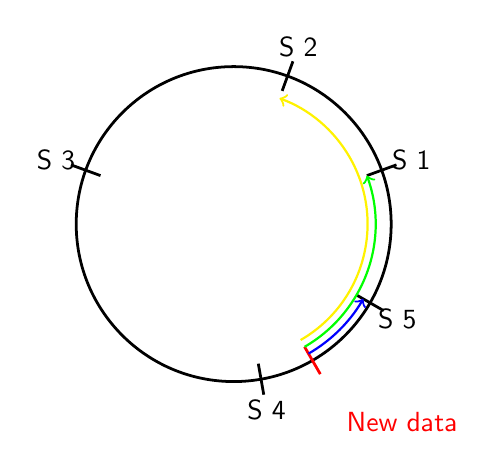
\begin{tikzpicture}
\foreach \a [count=\ai] in {20, 70, 160, 280, 330}{
  \draw (\a:1.8cm) -- (\a:2.2cm); 
  \node (s\ai) at (\a:2.4cm)  {S \ai};
}

\draw (0,0) circle (2cm);

\draw [red] (300:1.8cm)  -- (300:2.2cm); 
\node [red, anchor=north west] (data) at (300:2.6cm) {New data};
\draw [blue, ->, thick]  (300:1.9cm) arc  (300:330:1.9cm); 
\draw [green, ->, thick]  (300:1.8cm) arc  (300:20+360:1.8cm); 
\draw [yellow, ->, thick]  (300:1.7cm) arc  (300:70+360:1.7cm); 

\end{tikzpicture}


\end{document}